\documentclass[a4paper,10pt,landscape,twocolumn]{article}
\RequirePackage{verbatim}
\RequirePackage{ifthen}
\RequirePackage{fancyhdr,fancyvrb}
\RequirePackage{url}

\RequirePackage{figlatex}
\RequirePackage{graphics}
\usepackage[utf8]{inputenc}

\usepackage[cm]{fullpage}
\setlength{\oddsidemargin}{-2cm}
\setlength{\evensidemargin}{-1cm}
\addtolength{\topmargin}{-13mm}
\addtolength{\voffset}{-1cm}
\addtolength{\textheight}{35mm}
\addtolength{\textwidth}{2cm}
\setlength{\headsep}{25pt}
\setlength{\parindent}{0pt}

\newcommand{\Section}[1]{{\Large \textbf{#1}}}
\newcommand{\Subsection}[1]{{\textbf{#1}}}


\begin{document}

\twocolumn[\null\bigskip\centerline{\Huge Mémento pour le shell}]
\medskip

\Subsection{Se déplacer dans l'arborescence}

\begin{tabular}{|p{3cm}|p{10cm}|}\hline
\texttt{cd} \textit{rep} & Aller dans le répertoire \textit{rep}
\hfill (\textbf{c}hange \textbf{d}irectory)\\\hline
\texttt{ls} [-l]& Affiche le contenu du répertoire de travail (détails avec -l) \hfill (\textbf{l}i\textbf{s}t)\\
\texttt{ls} \textit{rep}& Affiche le contenu d'un répertoire\\\hline

\texttt{pwd}&  Affiche le répertoire de travail actuel \hfill (\textbf{p}rint \textbf{w}orking \textbf{d}irectory)\\\hline
\end{tabular}

\medskip\Subsection{Manipulation de base des fichiers et répertoires}

\begin{tabular}{|p{3cm}|p{10cm}|}\hline
  \texttt{cp} \textit{fich1} \textit{fich2} & Copier un fichier sous un  
  nouveau nom \hfill (\textbf{c}o\textbf{p}y)\\
  \texttt{cp} \textit{fich1} \textit{fich2} \textit{rep} & Copier des fichiers 
  à un nouvel emplacement\\\hline
  \texttt{mv} \textit{fich1} \textit{fich2} & Renommer un fichier \hfill (\textbf{m}o\textbf{v}e)\\
  \texttt{mv} \textit{fich1} \textit{fich2} \textit{rep} & Déplacer des fichiers vers un nouvel
  emplacement\\\hline

\texttt{rm} \textit{fich}&Effacer un fichier  \hfill (\textbf{r}e\textbf{m}ove)\\
\texttt{rmdir} \textit{rep}&Effacer un répertoire (doit être vide) \\
\texttt{rm -r} \textit{rep}&Effacer une arborescence (attention, pas de garde-fou)\\\hline

\texttt{mkdir} \textit{rep} & Créer un nouveau répertoire \textit{rep} \hfill
(\textbf{m}a\textbf{k}e \textbf{dir}ectory)
\\\hline

\texttt{chmod} \textit{droits} \textit{fich}& Change les droits, les permissions
du fichier \hfill(\textbf{ch}ange \textbf{mod}e)\\\hline
\texttt{less} \textit{fichier}& Lire un fichier à l'écran ('h' pour l'aide, 'q' pour quitter)\\\hline

\end{tabular}

\medskip\Subsection{Aide en ligne}

\begin{tabular}{|p{3cm}|p{10cm}|}\hline
\texttt{man} \textit{commande} & Affiche la page de manuel de la
 \textit{commande}\\\hline
%man 2 \textit{syscall} & Affiche la documentation de l'appel système 
%\textit{syscall}\\
\texttt{man 3} \textit{fonction} & Affiche la documentation de la
 \textit{fonction}\\\hline
\texttt{help test}& Aide interne de bash, sur les tests\\\hline
\end{tabular}

\medskip\Subsection{Contrôler les processus en cours d'exécution}

\begin{tabular}{|p{3cm}|p{10cm}|}\hline
C-c & Interrompe (tue) le programme en cours \\\hline
C-z & Suspend (endort) le programme en cours \\\hline

\texttt{fg ; bg} & Relance  tâche interrompue (premier/arrière plan)
 {\small \textbf{f}ore/\textbf{b}ack\textbf{g}round}\\\hline

\texttt{top ; ps} & Montre (interactivement ou non) les processus actifs\\\hline

kill \textit{pid}; killall \textit{nom}& Envoie un signal (tue) un
programme\\\hline

C-s/C-q & Stoppe/relance le défilement de l'affichage\hfill(\textbf{s}crolling)\\\hline
\end{tabular}

\medskip\Subsection{Manipulation avancée des fichiers}

\begin{tabular}{|p{3cm}|p{10cm}|}\hline
\texttt{find -name} \textit{``ab*''} & Cherche tous les fichiers dont le nom commence par ab \\\hline

\texttt{grep} \textit{motif} \textit{fichier}& Sélectionne les lignes du \textit{fichier}
contenant \textit{motif}\\\hline

  \texttt{sed s/}\textit{cherch}\texttt{/}\textit{rpl}\texttt{/}&
  Remplace le motif \textit{cherch} par \textit{rpl} dans le flux\\\hline 
\texttt{cat} \textit{fichier}& Affiche le \textit{fichier} à l'écran (pas interactif)\\ \hline

  \texttt{head -n 5} \textit{fichier}&
   Affiche les 5 première lignes de \textit{fichier} (\texttt{tail} pour la fin) \\\hline

%\texttt{tail} \textit{fichier}& Affiche la fin de \textit{fichier} (-f si \textit{fichier} grandit encore) \\\hline
%\texttt{wc} \textit{fichier} & Compte les caractères, les mots et les lignes du
% \textit{fichier}\\\hline
%\texttt{file} \textit{fichier} & Affiche le type de fichier (exécutable, texte, image,
%etc)\\\hline
\texttt{diff -u} \textit{fich1} \textit{fich2}& Affiche les différences entre les deux fichiers\\\hline
%\texttt{touch} \textit{fichier} &Créer ou changer la date de modification de \textit{fichier}\\\hline

{\small \texttt{tar cvfz} \textit{ar.tgz} \textit{rep}} & Crée une archive \textit{ar.tgz}
contenant le répertoire \textit{rep}\\
\texttt{tar xvfz} \textit{arch.tgz} & Ouvre l'archive \textit{arch.tgz}\\\hline

\texttt{gzip} \textit{f}; \texttt{gunzip} \textit{f.gz} & Compresse / Décompresse un fichier\\\hline
\end{tabular}

\medskip\Subsection{Convertions}\smallskip

\begin{tabular}{|p{30mm}|p{100mm}|}\hline
convert & Manipule et converti les fichiers d'image (paquet imagemagic)\\\hline
sox & Manipule et converti les fichiers de son\\\hline
mplayer & Manipule les fichiers vidéo\\\hline
\end{tabular}

\newpage

\Subsection{Raccourcis clavier de Bash}
\smallskip

\begin{tabular}{|p{6mm}|p{35mm}|p{6mm}|p{32mm}|p{10mm}|p{27mm}|}\hline
C-a& Aller en début de ligne& C-u& Coupe tout à gauche & C-l& Efface l'écran \\\hline
C-e& Aller en fin de ligne  & C-k& Coupe tout à droite & C-d& Quitte bash    \\\hline
TAB& Complétion auto.       & C-r& Recherche historique& S-up&Remonte l'écran \\\hline
\end{tabular}

\medskip\Subsection{Redirections de flux}

\begin{tabular}{|p{32mm}|p{10cm}|}\hline
\textit{programme} \verb+>+ \textit{fichier} &Sortie du \textit{programme} redirigée dans \textit{fichier}.\\\hline
\textit{programme} \verb+<+ \textit{fichier} &Le programme lit son entrée depuis le \textit{fichier}.\\\hline
\textit{programme}  \verb+>>+ \textit{fich}  &Sortie du \textit{programme} concaténée à la suite de \textit{fich}.\\\hline
\textit{progA} \verb+|+ \textit{progB}       &Sortie de \textit{progA} tubée en entrée de \textit{progB}.\\\hline
\textit{prog}  \verb+2>+ \textit{fichier}    &Le flux 2 (stderr) de \textit{prog} redirigée dans le \textit{fichier}.\\\hline
\textit{prog} \verb+2>>+ \textit{fichier}    &Le flux 2 (stderr) de \textit{prog} concaténée dans le \textit{fichier}.\\\hline
\textit{prog} \verb+2>&1+                    & Flux 2 (stderr) fusionné dans le flux 1 (stdout).\\\hline
\textit{prog} \verb+<<+ \texttt{marqueur}    & Entrée standard de \textit{prog} en place, jusqu'à la ligne \texttt{marqueur}\\\hline
\end{tabular}

\medskip\Subsection{Guillemets et quotes}

\begin{tabular}{|p{32mm}|p{10cm}|}\hline
\verb+\c+& Le caractère c, littéralement\\\hline
  \verb+`+\textit{commande}\verb+`+&
     Exécute \textit{commande} et place sa sortie sur la ligne\hfill(`: AltGr-7)\\\hline
'blabla' & Garde le blabla sans interpréter quoi que ce soit\hfill(': sous le 4)\\\hline
  "blabla" & Garde le blabla après avoir interprété les \verb+$+,
           \verb+`...`+ et \verb+\+\\\hline
\end{tabular}

\medskip\Subsection{Flôt de contrôle en shell}

\begin{tabular}{|p{25mm}|p{34mm}|p{25mm}|p{40mm}|}\hline
  \verb+cmd1 && cmd2+& ET entre commandes&\verb+var=value+& Affectation\\\hline
  \verb+cmd1 || cmd2+& OU entre commandes&\verb+$var+&Usage de la variable\\\hline

  \texttt{if} \textit{cmd} \texttt{; then}  \par
   ~~\textit{cmd;}\par
  \texttt{elif} \textit{\small cmd}\texttt{;then}\par
   ~~\textit{cmd;}\par
  \texttt{else}\par
   ~~\textit{cmd;}\par
  \texttt{fi}
  &
  \texttt{for} \textit{var} \texttt{in} \textit{list} \texttt{; do} \par
   ~~\textit{cmd;}\par
  \texttt{done}\par~\par
  \texttt{while} \textit{cmd} \texttt{; do}\par
   ~~\textit{cmd;}\par
    \texttt{done}
   &
   \verb+a{1,2,3}b+ \par~~\verb+= a1b a2b a3b+\par
   ~\par                    
   ~\par                    
   \verb+{1..5}+\par~~\verb+=1 2 3 4 5+                       
   & \textit{cmd} \verb+|+ \texttt{while read} \textit{line;} \texttt{do}\par
  ~~echo \$line\par
done

  \\\hline
  
\end{tabular}

\medskip\Subsection{Tests pour \texttt{if [ ... ]} (voir aussi help test})

\begin{tabular}{|p{13mm}|p{48mm}|p{13mm}|p{48mm}|}\hline
-r fich & Si droit de lecture sur \textit{fich} &
-w fich & Si droit d'écriture sur \textit{fich}\\
-x fich & Si droit d'execution sur \textit{fich} &
-e fich & Si \textit{fich} existe.\\
-f fich & Si \textit{fich} est un fichier standard&
-d fich & Si \textit{fich} est un répertoire.\\
{\small fA -nt fB} & Si fichier \textit{fA} modifié après \textit{fB}&
-s fich & Si taille supérieure à 0.\\\hline

A = B  & Si les chaînes \textit{A} et \textit{B} sont égales & 
A != B & Si \textit{A} et \textit{B} sont différentes \\
-z CH & Si la chaîne \textit{CH} est vide & -n CH & Si la chaîne \textit{CH} n'est pas vide\\\hline

{\small n1 -eq n2} & Si le nombre \textit{n1} est égal à \textit{n2}&
{\small n1 -ne n2} & Si $n1 \ne n2$\\
{\small n1 -lt n2} & Si $n1 < n2$ (less than)& 
{\small n1 -le n2} & Si $n1 \le n2$ (less or equal)\\
{\small n1 -gt n2} & Si $n1 > n2$ (greater than)&
{\small n1 -ge n2} & Si $n1 >= n2$ (greater or equal)\\\hline
{\small e1 -a e2}  & ET booléen entre expressions& 
{\small e1 -o e2}  & OU booléen entre expressions\\\hline

\multicolumn{4}{|l|}{\texttt{if [ $\backslash($ -f \$fich1 -a -r \$fich1 $\backslash)$ -o  $\backslash($ -f \$fich2 -a -r \$fich2 $\backslash)$ ] }}\\\hline
\end{tabular}

\url{http://johnstowers.co.nz/pages/bash-cheat-sheet.html}\\
\url{http://www.freeos.com/guides/lsst/}\\
\url{https://openclassrooms.com/courses/reprenez-le-controle-a-l-aide-de-linux}
%\end{document}
%%%%%%%%%%%%%%%%%%%%%%%%%%%%%%%%%%%%%%%%%%%%%%%%%%%%%%%%%%%%%%%%%%%%%%%%%%%%%%%%%%%%%%%%%%%%%%%%%%%%%%%
\newpage
\twocolumn[]
\null\bigskip\centerline{\Huge Mémento pour emacs}
\medskip

% \Subsection{Convention d'écriture}

% \begin{tabular}{|p{3cm}|p{10cm}|}\hline
%   C-\textit{x}& Appuyer simultanément sur les touches Ctrl et \textit{x}
%   \\\hline

%   M-\textit{x}& Appuyer simultanément sur les touches Alt et \textit{x} (ou
%   Esc puis \textit{x})
%   \\\hline

%   S-\textit{x}& Appuyer simultanément sur les touches Shift et \textit{x}
%   \\\hline

%   C-M-\textit{x}& Appuyer simultanément sur les touches Ctrl, Alt et \textit{x}
%   \\\hline

%   M-x \textit{commande}& Faire M-x puis taper la \textit{commande}
%   \\\hline

% \end{tabular}

Il faut installer \texttt{spacemacs} pour une bonne configuration par
défaut.\\
\url{http://sachachua.com/blog/2014/04/emacs-beginner-resources/}


\medskip\Subsection{Ouvrir et fermer des fichiers}

\begin{tabular}{|p{13mm}|p{48mm}|p{13mm}|p{48mm}|}\hline
  C-x C-c & Quitter& 
  C-z & Suspendre emacs \\\hline

  C-g     & Annuler la commande en cours &
  C-\_    & Défaire la dernière action \\\hline

  C-x C-f & Ouvrir un fichier & C-x k & Fermer un fichier \\\hline

  C-x C-s & Sauvegarder le fichier&
  C-x C-w & Sauvegarder sous un autre nom\\\hline

  C-x b   & Changer de fichier ouvert &
  C-x C-b & Liste des fichiers ouverts \\\hline
\end{tabular}

\medskip\Subsection{Chercher et remplacer}

\begin{tabular}{|p{13mm}|p{48mm}|p{13mm}|p{48mm}|}\hline
  C-s & Cherche plus bas & 
  C-r & Cherche plus haut \\\hline 
  M-\% & Cherche/remplace & 
  M-C-s & Cherche expression regulière \\\hline 
\end{tabular}

\medskip\Subsection{Déplacer le curseur}

\begin{tabular}{|p{13mm}|p{48mm}|p{13mm}|p{48mm}|}\hline
  gch & Un caractère à gauche & drt & Un caractère à droite \\\hline
  haut & Une ligne plus haut & bas & Une ligne plus bas \\\hline
  C-gch & Un mot à gauche & C-drt & Un mot à droite \\\hline
  M-\{ & Un paragraphe plus haut & M-\} & Un paragraphe plus bas \\\hline
  C-a & Début de ligne & C-e & Fin de ligne \\\hline
  M-$<$ & Début de fichier & M-$>$ &Fin de fichier \\\hline
%  M-g \textit{n}& Aller à la ligne \textit{n} &
%  C-M-a$|$e& Fonction précédente$|$suivante\\\hline
\end{tabular}

\medskip\Subsection{Manipulation et sélection de blocs et rectangles}

\begin{tabular}{|p{13mm}|p{48mm}|p{13mm}|p{48mm}|}\hline
  C-SPC & Place la marque ici & 
  C-x C-x & Inverse marque/pos. courante \\\hline 

  C-x & Coupe la sélection \hfill(aussi: C-w) & 
  C-x r k & Coupe le rectangle \\\hline 

  C-c & Copie la sélection \hfill(aussi: M-w) & 
  C-x r r & Copie le rectangle  \\\hline 

  C-v & Colle la sélection \hfill(aussi: C-y)& 
  C-x r y & Colle le rectangle \\\hline 

  C-k & Coupe la fin de la ligne &
  M-d & Coupe le prochain mot \\\hline
\end{tabular}

\medskip\Subsection{Avoir plusieurs fenêtres}

\begin{tabular}{|p{13mm}|p{48mm}|p{13mm}|p{48mm}|}\hline
C-x 2 & Coupe fenêtre horizontalement&C-x 3&Coupe la fenêtre verticalement\\
\hline

C-x 5 2 & Lancer une autre fenêtre & C-x o & Changer partie dans la fenêtre\\
\hline

C-x 1 & Fermer les autres fenêtres&C-x 0& Ferme la fenêtre 
courante \\\hline

C-x $<$ & Défille vers la gauche & C-x $>$ & Défille vers la droite\\\hline

\end{tabular}

\medskip\Subsection{Divers}

\begin{tabular}{|p{13mm}|p{48mm}|p{13mm}|p{48mm}|}\hline
  TAB & Réindente la ligne &
  M-q & Réindente le paragraphe\\\hline

  M-/ & Complète le mot & M-\$ &Vérifie orthographe du mot\\\hline
  M-! & Exécute une commande shell & {\small M-x shell} & Ouvre un
  shell\\\hline

  C-h t & Affiche le tutoriel & C-h i & Entre en mode info\\\hline
\end{tabular}

\bigskip\Subsection{Modes utiles pour emacs}

\begin{tabular}{|p{27mm}|p{103.5mm}|}\hline
  auctex& Environnement complet pour le \LaTeX\\\hline
  org-mode& Environnement pour tout organiser\\\hline
  flyspell-mode& Correction orthographique à la volée\\\hline
\end{tabular}

\newpage


\null\bigskip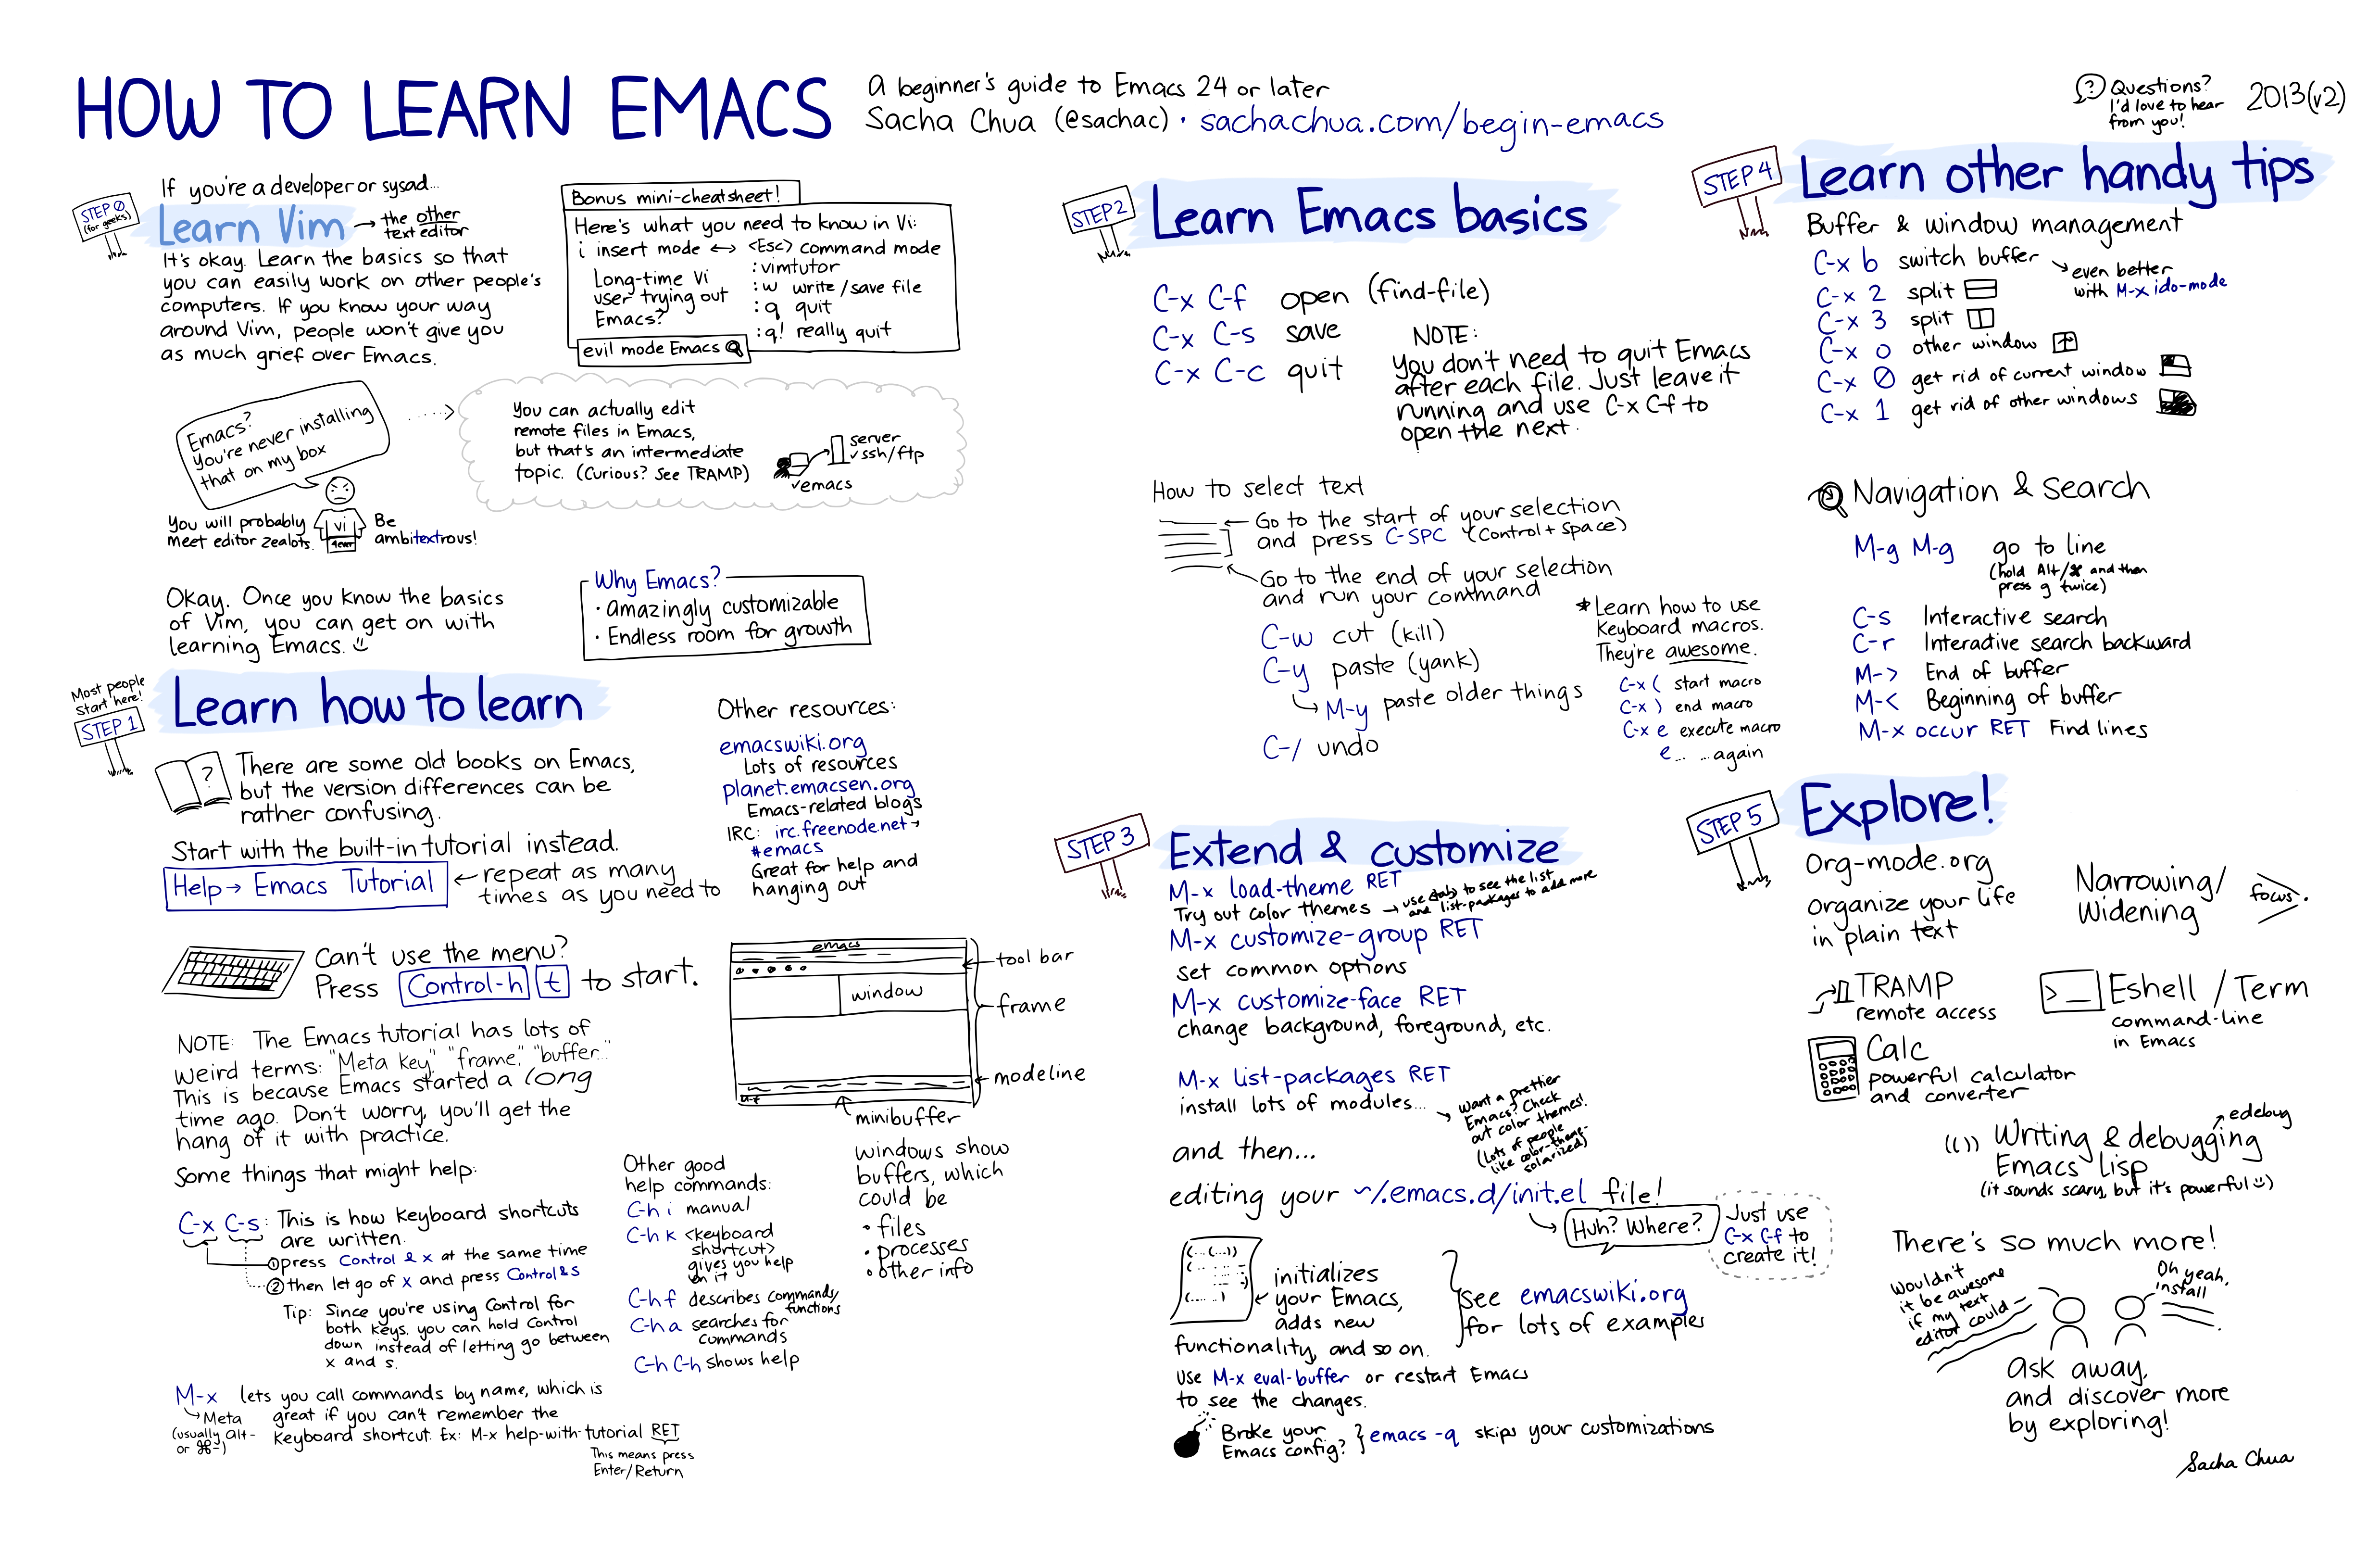
\includegraphics[width=1.37\linewidth,angle=90]{How-to-Learn-Emacs-v2-Large.png}

\end{document}

Todo shell:
   http://www.johnstowers.co.nz/blog/pages/bash-cheat-sheet.html
 - ${bah}
 - pattern matching ?
 - les droits de chmod ?

http://sachachua.com/blog/wp-content/uploads/2013/05/How-to-Learn-Emacs-v2-Large.png

%%% Local Variables:
%%% coding: utf-8
